\documentclass[draft]{agujournal2019}
\usepackage{url}
\usepackage{lineno}
\usepackage{soul}

\linenumbers
\draftfalse
\journalname{Earth and Space Science}


\begin{document}

\title{AuroraX, aurorax-api (or pyaurorax?), and aurorax-asilib: a user-friendly auroral all-sky imager analysis framework}

\authors{M. Shumko\affil{1, 2}, B. Gallardo-Lacourt\affil{1,2}, A.J. Halford\affil{1}, E. Donovan\affil{3}, E.L. Spanswick\affil{3}, D. Chaddock\affil{3}, I. Thompson, and K.R. Murphy}

\affiliation{1}{NASA's Goddard Space Flight Center, Greenbelt, Maryland, USA}
\affiliation{2}{Universities Space Research Association, Columbia, Maryland, USA}
\affiliation{3}{University of Calgary, Calgary, Alberta, Canada}

\correspondingauthor{M. Shumko}{msshumko@gmail.com}


\begin{keypoints}
\item AuroraX and aurorax-api are online interfaces to quickly visualize the aurora and calculate conjunctions
\item aurorax-asilib is a companion Python package for detailed analysis of auroral all-sky imager data 
\item Together, these tools enable effortless end-to-end discovery and analysis of the aurora
\end{keypoints}


\begin{abstract}
Here we introduce the AuroraX project which consists of open-source software designed to effortlessly discover and analyze auroral imager data. At this time AuroraX consists of three main tools: the AuroraX website (\url{https://aurorax.space/}); aurorax-api, a application program interface to the AuroraX website written in Python; and aurorax-asilib, an auroral all-sky imager library also written in Python. Together, these three tools enable a rapid and painless end-to-end analysis of the aurora. One such example is a conjunction study: AuroraX---or the aurorax-api---can be used to quickly identify conjunctions between numerous ground- and space-based instruments and quickly look at keograms from the available imagers to determine what the imagers observed. A list of conjunctions, together with aurorax-asilib, can be then used to download, load, and analyze all-sky imager data directly on a personal computer.
\end{abstract}


\section*{Plain Language Summary}
\noindent The aurora is a ubiquitous light spectacle that has been observed in the polar regions for millennia. The regional scale of the aurora has led to the development of numerous imagers, and arrays of imagers, that continuously take images thorough the night. The image volume has quickly become unimaginable by any group of scientists, so the imager datasets are at best fragmented on the internet, and at worst hidden from the public. The AuroraX project aims to combine the publicly-available datasets into one easily accessible location. This project consists of three main tools:  the AuroraX website (\url{https://aurorax.space/}); aurorax-api, a application program interface to the AuroraX website written in Python; and aurorax-asilib, an auroral all-sky imager library also written in Python. Together, these three tools make the auroral data easily accessible and to the public and the scientific community---so that we can all enjoy and wonder the beautiful spectacle of the aurora.


\section{Introduction}\label{intro}
\textcolor{blue}{
      OUTLINE
      \begin{itemize}
            \item Brief history of ASIs and ASI arrays. Talk about why THEMIS ASI exists. Discuss CANOPUS? Linage.
            \item Breadth of possible science questions that can be answered with aurora image data.
            \item Problem: modern ASI arrays produce an immense volume of data.
            \item Why this software? Aurora ASI data formats very greatly, each with their own caveats. This centralized software package is maintained by the AuroraX team. 
            \item Benefits: Maintained by the AuroraX team so it's usability is of paramount importance
            \item Reduce the barrier to entry into auroral physics. Reduce the technical requirements and  enable rapid discovery of new science.
            \item Instead of case study results, larger statistical behavior will likely appear.
            \item remove the need for scientists needing to write duplicate code to use these popular missions. AS a result, this will enable scientists to dive right into the science and not need to know the details of data management (downloading and loading data, as well as applying routine data processing steps
      \end{itemize}
}

Since the 1960s the space physics community has utilized optical ground-based instrumentation that has led to discoveries and from which great advancements in the field have been derided. Some of these discoveries include the early description of a substorm introduced by Akasofu (1964), and several descriptions of new phenomena that highlight the tight connections between the magnetosphere and ionosphere (e.g., ). 

Meridian Scanning photometers (MSP), such as the Canadian Auroral Network for the OPEN (Origins of Plasmas in Earth's Neighborhood) Program Unified Study (CANOPUS) array, were first utilized for remote sensing the high-latitude ionosphere (e.g., Rostoker et al. 1985). These MSPs were later followed by two dimensional All-sky Imagers (ASIs) that took the space physics field into a deeper understanding of the ionosphere-magnetosphere coupled system. In the present day, the space physics community has carried a long legacy of ground-based optical instruments, with perhaps the THEMIS-ASI observatories being one of the most successful ones. Currently, many different optical arrays are in operation or are in development (e.g., THEMIS-ASI, REGO, MANGO, TREx, PWING, among others). These modern ASIs work continuously in high temporal and spatial resolution, where each camera produces thousands of images per night.

The rapidly increasing volume of imager data, together with unique data formats, significantly burdens space physicists with mundane and duplicated software engineering tasks---download data, load and correctly parse the data, etc. This unnecessary burden can also lead to mistakes in analysis software that may require unnecessary troubleshooting time from the ASI team, or more worrisome---publish inaccurate findings that mislead researchers and the public. Thus, robust auroral analysis tools are required.

We introduce the AuroraX project that aims to overcome the above issues by providing three robust tools that most auroral researchers need. The first tool is the AuroraX website (https://aurorax.space/) that can quickly plot keograms, show what imagers operated at a given time, and calculate conjunctions between numerous ground- and space based instruments. The second tool is the aurorax-api, a Python library that interfaces with the AuroraX website to download the data to a personal computer and automate those tasks. The third tool is aurorax-asilib, a Python all-sky imager library. aurorax-asilib provides functions to the download, load, analyze, and visualize THEMIS and REGO ASI data. 

\section{AuroraX}\label{aurorax}
\textcolor{blue}{
      OUTLINE
      \begin{itemize}
            \item What is it?
            \item A highly optimized conjunction search
            \item On-demand keograms
            \item Virtual Observatory
            \item pyaurorax (aurorax-api) to directly access AuroraX services.
            \item Figure 1: a) a screenshot of the nightly keograms, b) screenshot of the conjunction search tool. 
      \end{itemize}
}

\subsection{Website}
The AuroraX website, located at (\url{https://aurorax.space/}).

\subsection{aurorax-api}
The AuroraX servers can also send data to a user's personal computer without an internet browser using a Python Application Program Interface (API) called aurorax-api. The aurorax-api handles the payload (transmitted messages) format so you don't have to. The \verb|pyaurorax.ephemeris| module contains software to download and upload the satellite ephemeris.

\begin{figure}
      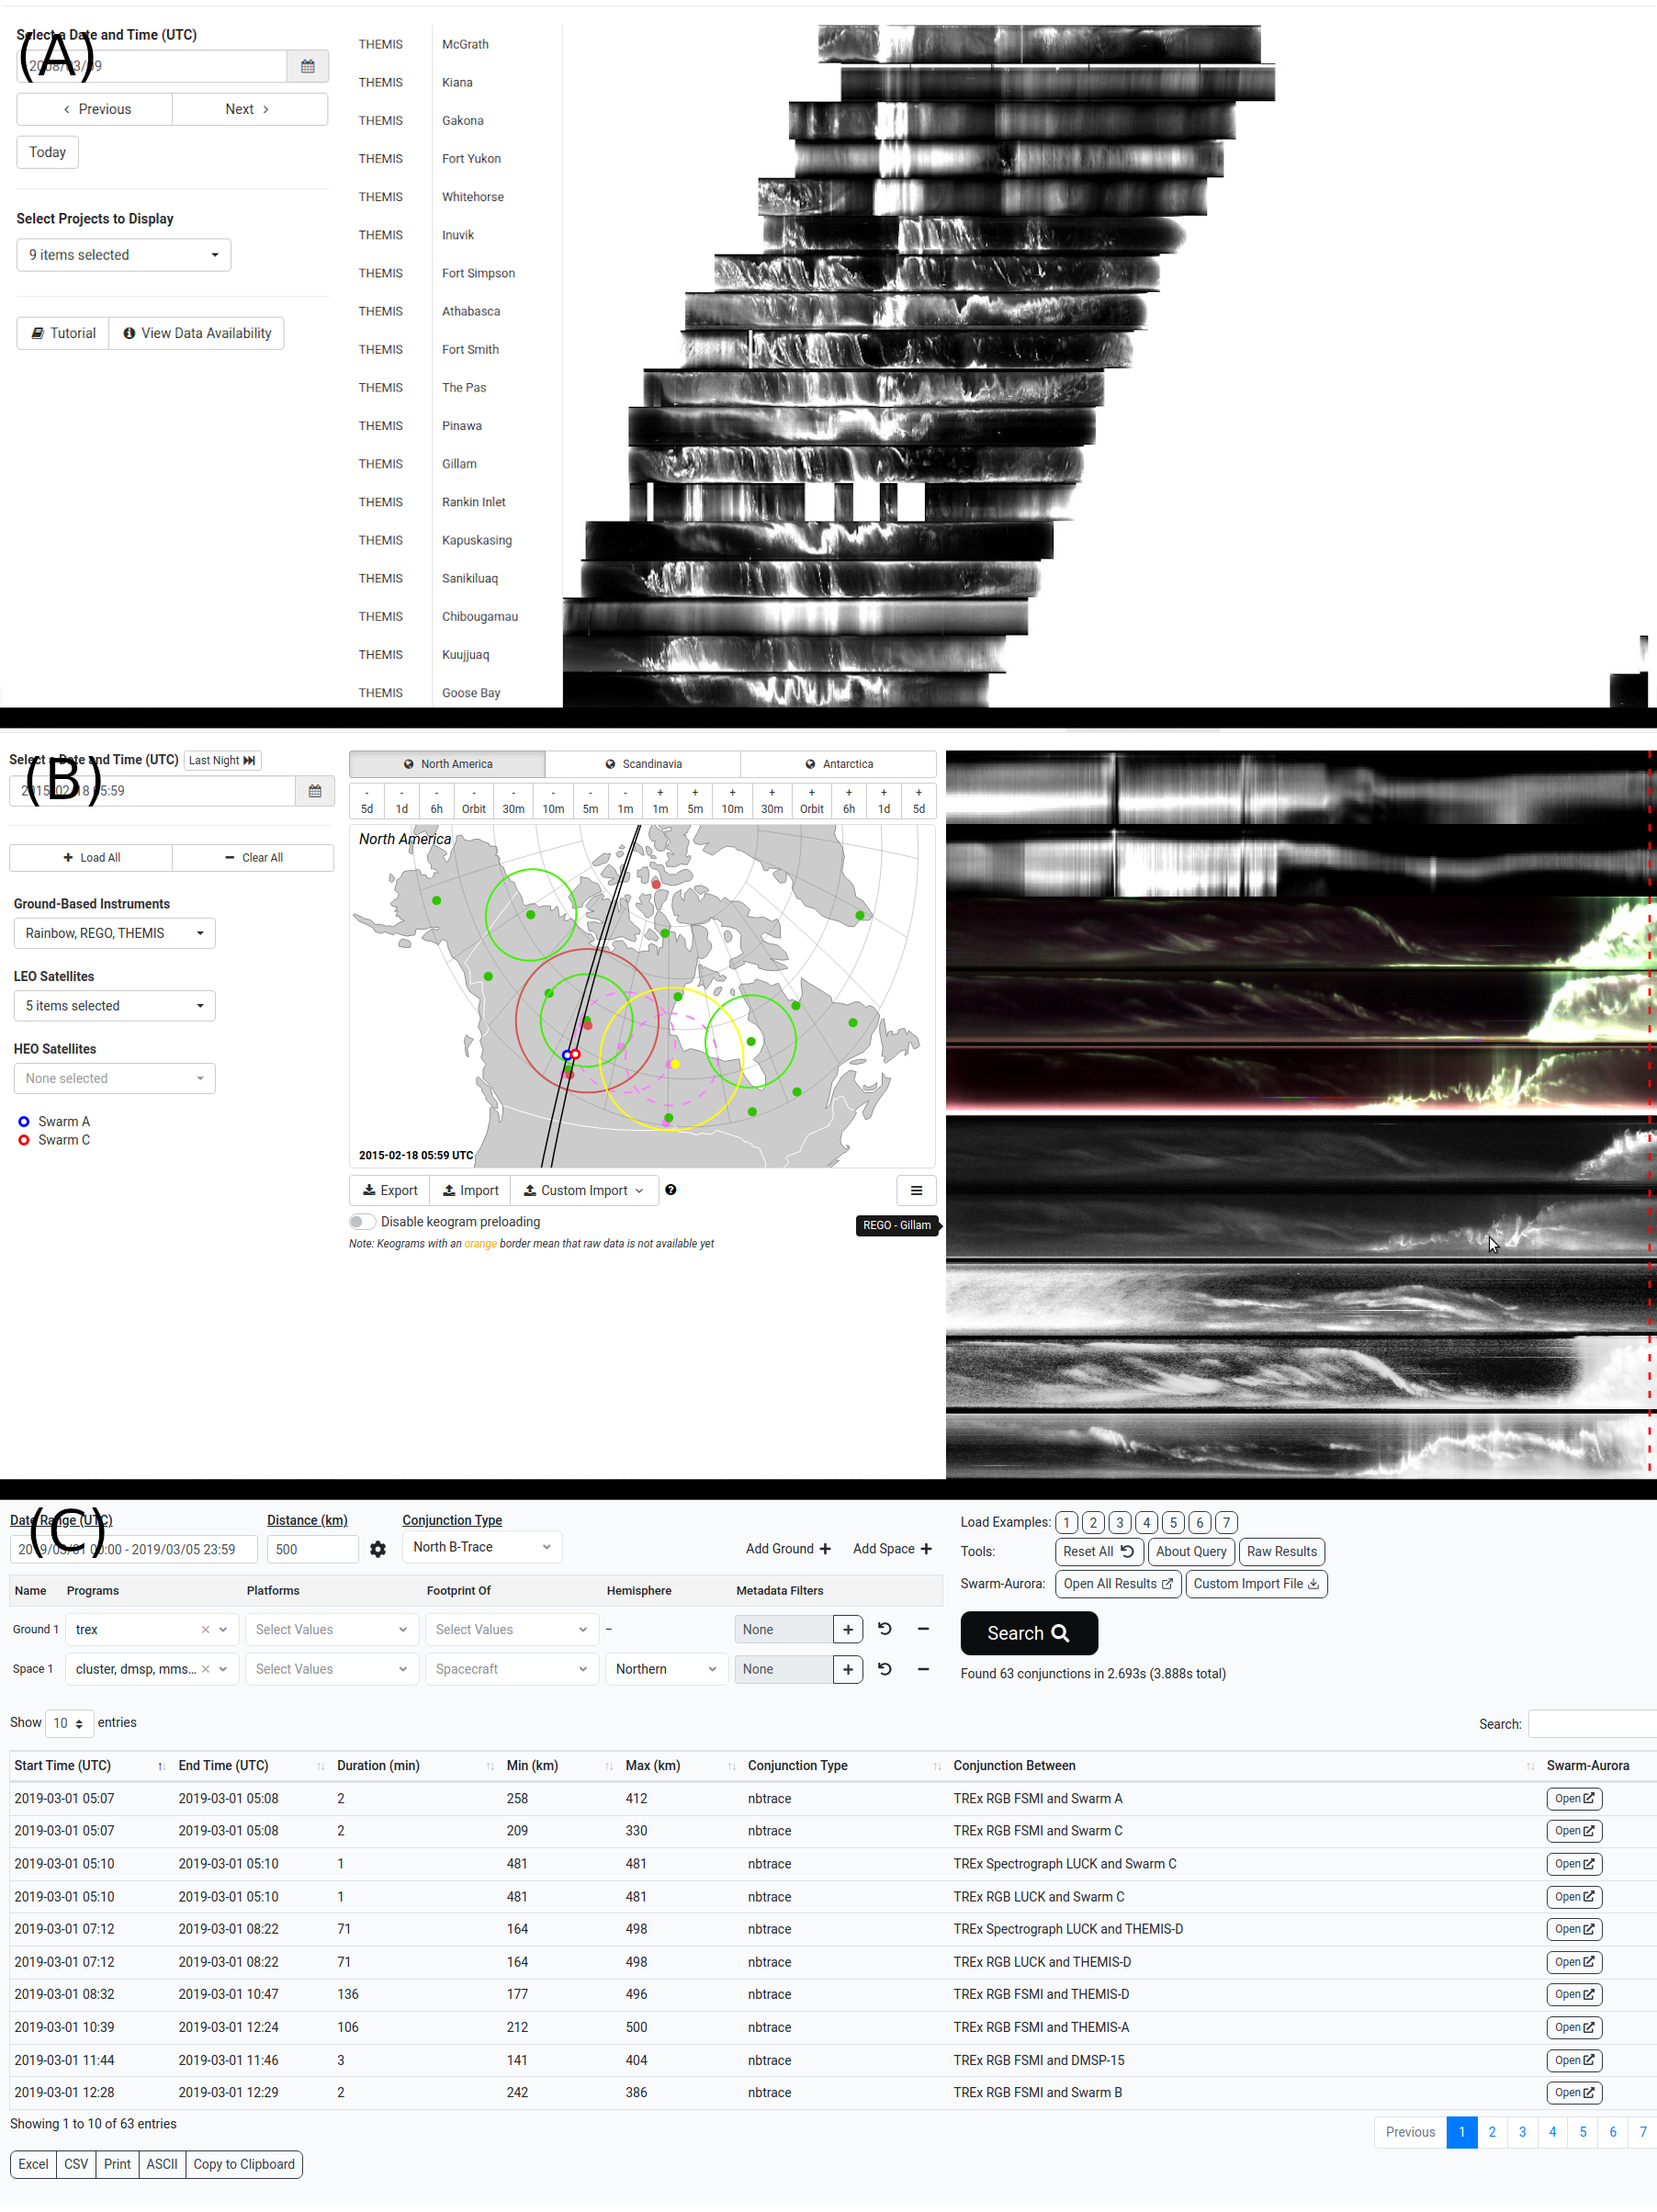
\includegraphics[width=\textwidth]{figures/fig1.png}
      \caption{The \url{https://aurorax.space/} interface. Panel a shows the daily keogram browser. Panel b shows the conjunction finder with keograms. And lastly, panel c shows the conjunctions in list form.}
      \label{fig1}
\end{figure}

\section{aurorax-asilib}\label{aurorax-asilib}
\textcolor{blue}{
      OUTLINE
      \begin{itemize}
            \item What is it? A Python library that helps researchers analyze THEMIS and REGO ASI images.The main functions are summarized in Table 1. It is designed to be simple and runnable on personal machines (relatively low memory usage). We strived to strike a balance between complicated and user-friendly tools.
            \item A table of function names and one sentence to describe their functions.
            \item The large file sizes lead to relatively long processing time. This is a fact that can be partly mitigated by an SSD. 
            \item Plug-in based architecture that allows new ASI arrays to be added and called by the core aurorax-asilib software.
      \end{itemize}
}

aurorax-asilib allows researchers to analyze ASI data on a PC. It provides a set of functions for common data analysis tasks using ASI data. Here we overview the functions and the online documentation has more examples, a tutorial, and a thorough API reference \url{https://aurora-asi-lib.readthedocs.io/}

As we tour the asilib functions, keep in mind that asilib is designed to help you with the lower-level tasks. For example, if you want to load the image data via \verb|asilib.load_image()|, asilib will attempt to download it if it is not already saved on the PC. Likewise, if you call \verb|asilib.plot_keogram()|, it will automatically load (and optionally download) the ASI data for you. Lastly, Figs. 2-4 were made using the code in a Jupyter Notebook that is provided with this article (in both the ipynb and pdf formats).

\subsection{Download and load ASI image and skymap data}
\textcolor{blue}{
      OUTLINE
      \begin{itemize}
            \item Handles the downloading and loading of ASI images. Main design principle: Ultimately, ASI image files consists of time stamps and images, so the asilib functions really only need to return that data
            \item Similarly with skymap calibration files
            \item If a file is already downloaded, you do not need an internet connection to work with the data
      \end{itemize}
}

Let us start with the four functions that download and load ASI image and skymap data: 

\begin{itemize}
      \item \verb|asilib.download_image()|,
      \item \verb|asilib.download_skymap()|,
      \item \verb|asilib.load_image()|, and
      \item \verb|asilib.load_skymap()|
\end{itemize} that are described below.

The \verb|asilib.download_image()| function downloads the level 1 hourly Common Data Format (CDF) files from \url{http://themis.ssl.berkeley.edu/data/themis/thg/l1/asi/} for THEMIS, and \url{http://themis.ssl.berkeley.edu/data/themis/thg/l1/reg/} for REGO. The files are saved in the \verb|asilib.config['ASI_DATA_DIR']| directory that at \verb|~/asilib-data/| be default, and is customizable.

The \verb|asilib.download_skymap()| function downloads all of the skymap files from \url{https://data.phys.ucalgary.ca/sort_by_project/THEMIS/asi/skymaps/} and \url{https://data.phys.ucalgary.ca/sort_by_project/GO-Canada/REGO/skymap/} for a given set of \verb|asi_array_code| and \verb|location_code|. The skymap files are in the Interactive Data Language (IDL) \verb|.sav| file format. Noteworthy is that \verb|asilib| downloads all of the skymap files for a given imager because the skymaps are only valid for a set time period (typically a year; see the logic for \verb|asilib.load_skymap()| that is described below).

As the name implies, \verb|asilib.load_image()| loads into memory and returns the ASI time stamps and images for a specified imager. This function loads both single and multiple images: a single time stamp and image if \verb|time| is provided, and an array of time stamps and images if \verb|time_range| is provided. As previously mentioned,\verb|asilib.load_image()| will try to download an hourly CDF file if it does not exist locally.

\verb|asilib.load_skymap()| is the last noteworthy input function; it loads the relevant skymap file into memory and returns the data in a dictionary. A relevant skymap file is the latest one before the specified \verb|time|. As with \verb|asilib.load_image()|, \verb|asilib.load_skymap()| will attempt to download the skymap functions if they are not already downloaded.

Before we discuss the plotting functions, we emphasize that the \verb|asilib.download_image()| and \verb|asilib.download_skymap()| functions are often unnecessary to call since they are called by \verb|asilib.load_image()| and \verb|asilib.load_skymap()|. However, the download functions are very useful if you need to download ASI image and calibration data in bulk---useful to analyze data offline, for example.

\subsection{Plotting single images}

The \verb|asilib| provides two ways to plot a single ASI image:

\begin{itemize}
      \item \verb|asilib.plot_fisheye()| and
      \item \verb|asilib.plot_map()|.
\end{itemize}

One common way to visualize all-sky images is with \verb|asilib.plot_fisheye()|. It plots the raw ASI images oriented with North at the top and East to the right of each image. The term fisheye comes from the fisheye lens that expands the imager's field of view to nearly $180^\circ$. For reference, the \verb|azel_contours| keyword argument superposes contours of elevation and azimuth in the fisheye image. Figure \ref{fig2}a,c show an example of an auroral arc observed concurrently by the THEMIS and REGO ASIs stationed at Rankin Inlet (RANK). If you don't override the parameters, the color map is automatically chosen: black-to-white for THEMIS and black-to-red for REGO. Also the color scale is dynamically calculated using percentile logic described in the documentation.

Another common way to visualize images is by projecting the fisheye image onto a geographic map using \verb|asilib.plot_map()|. asilib uses the skymap files to map each pixel's vertices to a (latitude, longitude) point at an assumed aurora emission altitude (typically 110 km for THEMIS and 230 km for REGO). Figure \ref{fig2}b,d show the fisheye images mapped to 110 km altitude. By default, pixels that look at $< 10^\circ$ elevations are not mapped due to the stretching of pixels closest to the horizon. And lastly, \verb|asilib.plot_map()| provides default map styles that can be overwritten by your custom \verb|cartopy| map passed in via the \verb|ax| keyword argument.

\begin{figure}
      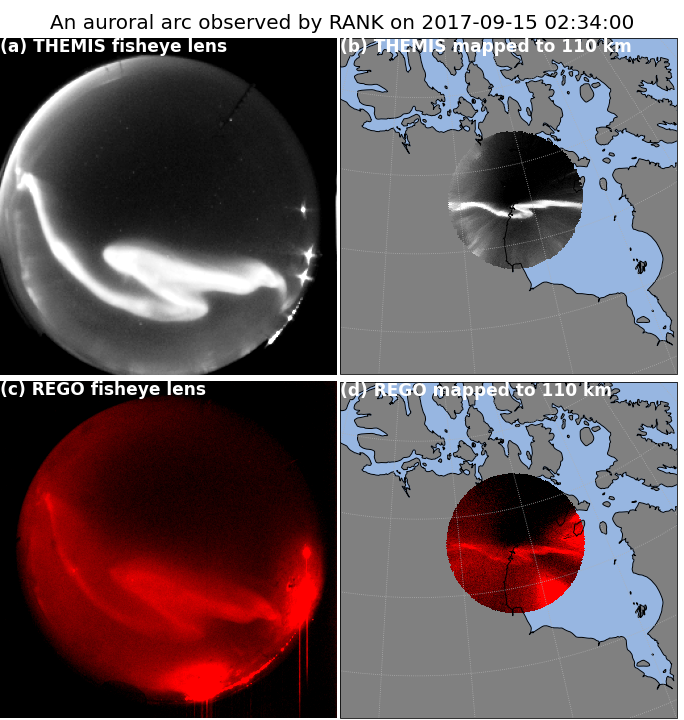
\includegraphics[width=\textwidth]{figures/fig2.png}
      \caption{ASI image of an auroral arc taken simultaneously by the REGO and THEMIS imagers at Rankin Inlet, Canada. Panels and a and c show the raw fisheye lens view, while panels b and d show the same images projected to the 110 km assumed aurora emission altitude. Only the pixels with $>10^\circ$ elevation are plotted.}
      \label{fig2}
\end{figure}

\subsection{Keograms}
A ubiquitous way to visualize ASI images and identify different types of aurora is with keograms. A keogram is a compression of many sequential ASI images into a single image showing pixel intensity as a function of latitude and time. Typically, they are assembled by looping over every image and slicing pixels that are oriented North-South through zenith (or through a custom path such a path of a stellite). Keograms are an essential tool that compress the information contained in hours of images into one plot. Objects in the sky such as auroral arcs, pulsating aurora, substorms, clouds, the moon, etc. all have unique keogram signatures that allow you to quickly classify what the imager observed. 

You can make a keogram using the \verb|asilib.plot_keogram()| function (that in turn calls \verb|asilib.keogram()|). Similar to \verb|asilib.plot_map()|, \verb|asilib.plot_keogram()| takes an optional \verb|map_alt| keyword argument. If it is not provided, the keogram's vertical axis is pixel index, but if a valid map altitude is provided, the vertical axis is geographic latitude. To minimize the PC's memory usage, \verb|asilib.keogram()| loads image data using \verb|asilib.load_image_generator()| that loads one image file at a time. The keogram shown in Fig. \ref{fig3} shows the dynamic nature of the aurora. Furthermore, the latitude  mapping transformation between panels a and b is substantial---low elevation pixels map to much wider sections of latitude as compared to the pixels near zenith.

\begin{figure}
      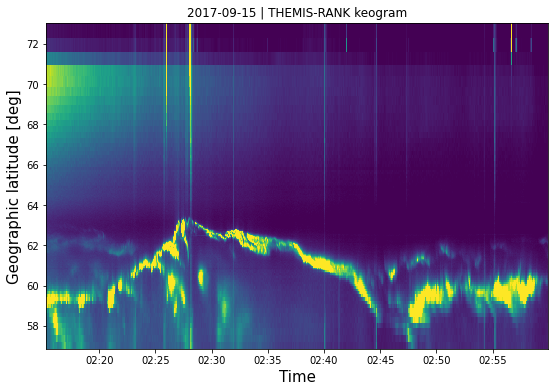
\includegraphics[width=\textwidth]{figures/fig3.png}
      \caption{A full-night keogram showing the dynamic aurora observed at Gillam, Canada. Panel a shows the unmapped keogram with the pixel index vertical axis, while panel b shows the latitude of the pixels mapped to 110 km altitude.}
      \label{fig3}
\end{figure}


\subsection{Animating Images}
You can easily animate ASI fisheye images using \verb|asilib.animate_fisheye()|. It first saves png images in a unique subfolder in the \verb|~/asilib-data/movies/images/| folder, and then animates them using the \verb|ffmpeg| library. Movie S1 in the supporting information (SI) document shows an example of \textcolor{red}{X type of aurora}.

Animating just the fisheye images is somewhat limiting. Thus, \verb|asilib| also includes \verb|asilib.animate_fisheye_generator()| (which is technically a coroutine) to iterate over and pause after each ASI image to allow you to modify it. Then, after the iteration is complete, \verb|asilib.animate_fisheye_generator()| combines the modified images into a movie. What sort of modifications can you make? For example, you can use it to superpose a satellite path and estimate the auroral intensity at its footprint during a conjunction. This is further described in the next two sections.

As the names imply, \verb|asilib.animate_map()| and \verb|asilib.animate_map_generator()| animate the projected images on a map. You can use them as easily as the \verb|animate_fisheye| functions. 

We mentioned earlier that the \verb|asilib.animate_fisheye_generator()| is technically a coroutine. So what does that mean? In this context, it means that before looping over each ASI image, you can request the images and time stamps from \verb|asilib.animate_fisheye_generator()| using the \verb|.send("data")| method. This approach appears rather contrived, however, a major advantage of this design is that the user sees exactly what ASI data the generator function will loop over. This is useful, for example, if you need the ASI time stamps to appropriately sample the images, plot the satellite location, and calculate the mean intensity of the aurora along the satellite trajectory. We will discuss this application later.

\subsection{ASI analysis tools}
Currently, \verb|asilib| provides three analysis functions that are useful for conjunction analysis: \verb|asilib.lla2footprint()|, \verb|asilib.lla2azel()|, and \verb|asilib.area2pixels()|.

\verb|asilib.lla2footprint()| uses IRBEM-Lib (CITE; requires a separate installation and compilation of the Fortran source code) to trace a satellite's position, in (latitude, longitude, altitude) (LLA) coordinates, along a magnetic field line. This field line is defined using one of the magnetic field models that are supported by IRBEM. The primary use of this function is to map a low Earth orbiting satellite's location at, say, 500 km altitude, to its magnetic footprint at the assumed auroral emission altitude, e.g. 110 km for THEMIS or 230 km for REGO as previously mentioned.

The next function is \verb|asilib.lla2azel()|. It maps the satellite's footprint location, in LLA coordinates, to the ASI's (azimuth, elevation) coordinates (AzEl) using the \verb|FULL_AZIMUTH| and \verb|FULL_ELEVATION| skymap arrays. This function returns both the AzEl coordinates as well as the corresponding pixels in the image.

And the last analysis function that we describe here is \verb|asilib.area2pixels()| that calculates a pixel mask of pixels inside an area. This function is useful to calculate the mean ASI intensity (or another statistical method) using pixels that map to a physical area in the sky. The mask has 1s inside of the area and \verb|numpy.nan| outside of it. You multiply the image with the mask: the pixel intensities outside of the area are then \verb|numpy.nan| and unchanged in the area. We chose to use \verb|numpy.nan| to ensure that the mean of the intensity is correctly applied---it will fail if you call \verb|numpy.mean(image*mask)|, but \verb|numpy.nanmean(image*mask)| will ignore NaNs and correctly calculate the mean intensity inside the area)

If you give it one LLA coordinate, the mask will have the same shape as the ASI image. On the other hand, if you pass multiple LLA coordinates, the mask's will have a new first dimension corresponding to the number of coordinates.

By default, the area is 5x5 km. If the area is so small that not even one pixel is contained inside it (but it is above the horizon), \verb|asilib.area2pixels()| will slowly increase the area tolerance until at least one pixel is found. Lastly, if the area is completely outside of the skymap, \verb|asilib| will raise a warning and the corresponding mask will be all NaNs. 

\subsection{An example: a satellite-ASI conjunction}\label{satellite_conjunction}
In this example we combine the aforementioned analysis functions into an example of a conjunction between a THEMIS ASI and a fictional satellite in 500-km altitude low Earth orbit. We will calculate and show the mean ASI intensity in a 20x20 km area, at 110 km altitude, around the satellite footprint and animate it.

First, to make this plot we use the satellite's location in LLA coordinates and time stamps. Here we use an imaginary satellite trajectory. In reality, the satellite and ASI time stamps are unlikely to line up, so you'll need to interpolate the satellite locations to the ASI time stamps.

We proceed with the analysis with three main steps. In step 1 we map the satellites position to 110 km using \verb|asilib.lla2footprint()|. In step 2, we calculate where in the sky (azimuth and elevation) the satellite's 110 km footprint was as a function of time using \verb|asilib.lla2azel()|. Lastly, in step 3 we calculate the pixels contained in a 20x20 km area at 110 km and calculate the mean ASI intensity in it using \verb|asilib.area2pixels()| and \verb|numpy.nanmean()|. Don't worry if this is hard to follow. These steps are implemented in the "Figure 4" section of the \verb|asilib_figures.ipynb| notebook.

Movie S2 shows the result of this conjunction analysis. Also, for a paper-friendly way to visualize the conjunction, Fig. \ref{fig4} shows a five-frame montage. Fig. \ref{fig4}a-d show the fisheye lens image at the annotated time stamp with the full satellite footprint path represented by the red line and the instantaneous footprint by the red dot. The yellow area shows what pixels are contained in a 20x20 km area surrounding the footprint. Lastly, Fig. \ref{fig4}e shows the mean ASI intensity time series for the conjunction---it clearly shows the signature of the auroral arc between 2:33:30 and 2:34:15.

\begin{figure}
      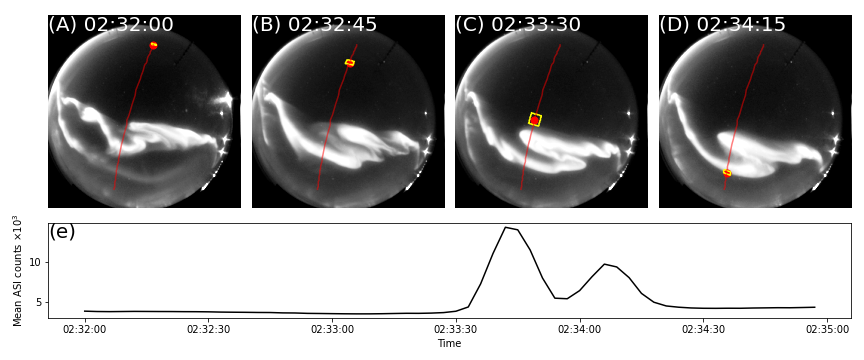
\includegraphics[width=\textwidth]{figures/fig4.png}
      \caption{A conjunction montage of Movie S2. Panels a-d shows the auroral arc evolution. The red line is the satellite track and the red dot is its instantaneous position. The yellow quadrilateral shows the pixels contained in a 20x20 km area at a 110 km altitude. Lastly, panel e shows the mean ASI intensity, as a function of time, inside the yellow quadrilaterals. When the satellite passed through the arc between 2:33:30 and 2:34:15, the ASI counts were enhanced.}
      \label{fig4}
\end{figure}

\section{Quality Assurance}
We developed \verb|asilib| with useability and maintainability at the forefront. The Python source code is available on \verb|aurora-asi-lib| GitHub repository \url{https://github.com/mshumko/aurora-asi-lib}. It is also archived on Zenodo and the Python Packaging Index (PyPI). On GitHub you can submit an Issue for bugs or feature requests, and you can contribute to \verb|asilib| using a Pull Request. 

Since documentation is critically important to the survival and usability of software, \url{readthedocs.org} hosts the \verb|aurora-asi-lib| documentation at \url{https://aurora-asi-lib.readthedocs.io/}. It contains installation instructions, examples, a comprehensive tutorial, and a detailed Application Programming Interface (API). The documentation source code is in the \verb|aurora-asi-lib/docs/| folder, useful in case a user needs to recreate the documentation on their computer with the Sphinx Python document generator.

To ensure code stability, the \verb|asilib| source code includes a few dozen unit and integration tests that you can run locally, and are automatically run on GitHub Actions every time a change is pushed to the repository. These tests test the main library functions and will quickly warn us if a proposed change broke anything.

Furthermore, we use semantic versioning and a \verb|CAHNGELOG.md| to communicate all major, minor, and patch changes with the community. We made many backward-incompatible changes before version 1.0.0, but henceforth we will indicate future backward-incompatible changes with major releases (i.e. version X.0.0). 

Lastly, the data format is integral to \verb|asilib|. The REGO and THEMIS data formats are fixed and are guaranteed to not change in the future.

% \section{Future Development}
% \textcolor{blue}{
%       OUTLINE
%       \begin{itemize}
%             \item Switch from CDF to pgm files.
%             \item Support more ASI arrays such as TREx
%             \item Community challenge. This package is made for the space physics community, so we will seek feedback (in the form of issues and bugs) that are discovered during a community challenge time period. 
%             \item Combine into a class architecture to share data. This is proving to be difficult to balance usability and maintainability.
%       \end{itemize}
% }
% While aurorax-asilib is feature complete, we plan to keep developing it.

\section{Conclusion}

\textcolor{blue}{
      OUTLINE
      \begin{itemize}
            \item AuroraX, aurorax-api, and aurorax-asilib tools provide the science community with a simple and a robust set of analysis tools
            \item Enable system-level science to be easily done
            \item Quickly sift through an immense volume of data to uncover new physics
            \item This is an end-to-end solution
            \item Plan to add support for other ASI arrays and satellites
            \item Help promote a uniform ASI data format for future cameras
            \item Add a paragraph to discuss the future work for this library includes...
      \end{itemize}
}
Hopefully we made a convincing case that AuroraX and aurorax-asilib are a useful set of tools to analyze the aurora. Our aim is to keep the implementation as simple as possible: enough for beginners who are starting to use this data, while also enabling sophisticated analysis.

AuroraX can be used anywhere with an internet connection. It is simple to use and it allows us to quickly identify times of interest (quickly as in during a lunch with collaborators in the middle of a conference).

aurorax-asilib, on the other hand, is designed to minimally use the internet. It only needs it to download the data. Once saved locally, aurorax-asilib allows you to easily make common aurora plots, and provides you with functions to get you the raw data if you need to implement something more sophisticated. We hope that the conjunction example demonstrates how useful aurorax-asilib functions are to transform your data and compare to the images.

For more information, see the AuroraX documentation at \url{https://docs.aurorax.space/} 

\acknowledgments
We are thankful for the engineers and scientists who made AuroraX, THEMIS ASI, and REGO ASI projects possible. M. Shumko and B. Gallardo-Lacourt acknowledge the support provided by the NASA Postdoctoral Program at the NASA’s Goddard Space Flight Center, administered by Universities Space Research Association under contract with NASA. The THEMIS and REGO ASI data is available from \url{https://data.phys.ucalgary.ca/}.

% \bibliography{refs.bib}

\end{document}